Ocorre em razão de mudanças na \textbf{geometria} dos elementos estruturais à medida que um carregamento é aplicado à estrutura.

Para que a influência da não-linearidade geométrica na análise de uma estrutura seja compreendida, é necessário entender o que são os \textbf{efeitos de segunda ordem}.

A condição de equilíbrio sempre foi considerada na configuração geométrica \textbf{inicial} da estrutura, isto é, na sua posição \textbf{não-deformada}. Esta análise se chama \textbf{Análise de primeira ordem} e os seus efeitos (deslocamentos e esforços resultantes) são chamados de \textbf{Efeitos de primeira ordem}.

Ao admitir o equilíbrio na configuração \textbf{indeformada}, passa-se a se fazer uma aproximação. Porém, na realidade, o equilíbrio de uma estrutura se dá \textbf{sempre} numa configuração \textbf{deformada}.

A análise do equilíbrio de uma estrutura na sua posição deformada é denominada de \textbf{Análise de segunda ordem} e os seus efeitos são chamados de \textbf{Efeitos de segunda ordem}.

A análise de 1ª ordem é uma aproximação que pode ser perfeitamente utilizada pelo fato de os efeitos de 2ª ordem, em muitos casos, \textbf{serem desprezíveis} (quando não apresentam acréscimo superior a 10\% nas solicitações em relação aos efeitos de 1ª ordem).

No entanto, existem certas situações em que os efeitos de 2ª ordem necessitam, obrigatoriamente, serem considerados, tais como:

\begin{itemize}
	\item Análise da estabilidade global;
	\item Cálculo dos esforços para dimensionamento dos pilares.
\end{itemize}

\begin{figure}[H]
	\begin{center}
	\caption{Efeitos de 1ª ordem à esquerda e Efeitos de 2ª ordem à direita.}
    	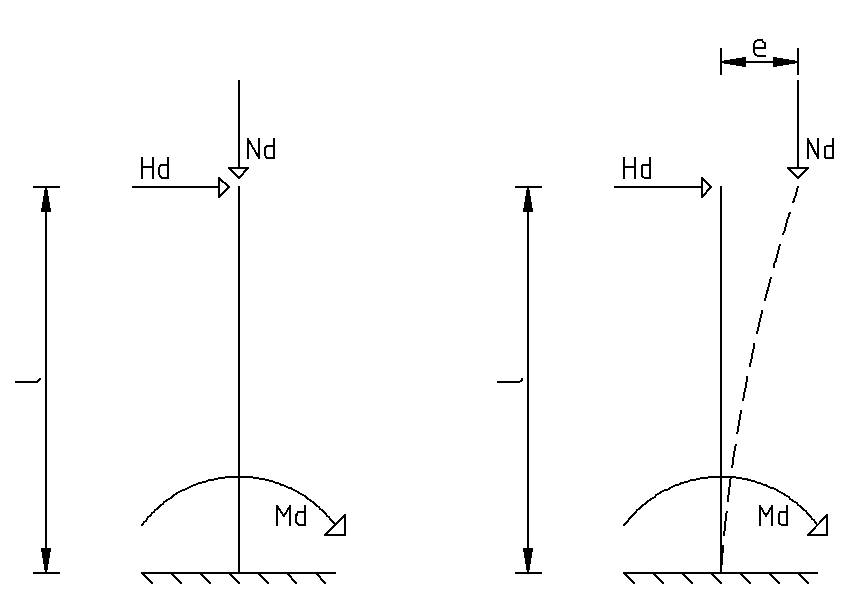
\includegraphics[width=0.5\textwidth]{Nao-linearidade-geometrica/Imagens/Efeitos-de-1a-e-2a-ordem.png}
	\end{center}
\end{figure}